\newif\ifvimbug
\vimbugfalse

\ifvimbug
\begin{document}
\fi

\exercise{Trajectory Generation with Dynamical Systems}
In this exercise we will use the Dynamic Motor Primitives (DMPs), described by the following dynamical system,
%
\begin{align}
    \ddot{y}&=\tau^2(\alpha(\beta(g-y)-(\dot{y}/\tau))+f_w(z)), \label{eq:dmp} \\
    \dot{z}&=-\tau\alpha_zz, \label{eq:dmp_phase}
\end{align}
%
where $y$ is the state of the system, $\dot{y}$ and $\ddot{y}$ are the first and second time derivatives, respectively. The attractor's goal is denoted by $g$ and the forcing function by $f_w$. The parameters $\alpha$ and $\beta$ control the spring-damper system. The phase variable is denoted by $z$ and the temporal scaling coefficient by $\tau$. The forcing function $f_w$ is given by
%
\begin{equation}
    f_w(z)=\frac{\sum_{i=0}^{K}\phi_{i}(z)w_{i}z}{\sum_{j=0}^{K}\phi_{j}(z)}=\vec{\psi}(z)^{T}\vec{w},
    \quad \textrm{with}\quad \psi_i(z) = \frac{\phi_i(z)z}{\sum_{j=1}^K\phi_j(z)},
\end{equation}
%
where the basis functions $\phi_i(z)$ are Gaussian basis given by
%
\begin{equation}
    \phi_i(z) = \exp(-0.5(z-c_i)^2/h_i),
\end{equation}
where the centers $c$ are equally distributed in the phase $z$, and the width $h$ is an open parameter. For the programming exercises a basic environment of a double link pendulum is provided, as well as the computation of the $\vec{\psi}_i(z)$.


\begin{questions}

%----------------------------------------------

\begin{question}{Similarities to a PD controller}{2}
Transform Equation~\eqref{eq:dmp} to have a similar structure to a PD-controller,
%
\begin{equation}
    \ddot{y}_z = K_P ( y^{des}_z - y_z ) + K_D ( \dot{y}_z^{des} - \dot{y}_z ) +
    u_{ff}
\end{equation}
%
and write down how the following quantities $K_p, K_d, y^{des}_z$ and $\dot{y}_z^{des}$ look like in terms of the DMP parameters. Do not expand the forcing function $f_w(z)$ at your solutions.

\begin{answer}
	$\ddot{y}=\tau^2 \alpha \beta (g-y) + (-\tau \alpha) (0-\dot{y}) +f_w(z)$	
	
	$K_P = \tau^2 \alpha \beta, \quad K_D= - \tau \alpha, \quad y_z^{des} = g , \dot{y_z}^{des}=0$
	\end{answer}

\end{question}

%----------------------------------------------

\begin{question}{Stability}{2}
Show why the DMPs are stable when $t\to\infty$ and what would the equilibrium point be.

\begin{answer}
	If you solve the diff. equation: $\dot{z}=-\tau\alpha_z z, \quad z(t)= z_0 e^{\lambda t}=z_0 e^{-\tau \alpha_z t} \overset{t \rightarrow \infty}{=}0 \rightarrow f_w(z) \overset{t \rightarrow \infty}{=}0 $.
	
	If you insert $f_w(z)=0$ in eq(1) you can calculate the equilibrium point by transforming eq. (1) with Laplace and then using the "Endwertsatz" or the steady state error.
	
	$G(s)=\frac{Y(s)}{g(s)}= \frac{\tau^2 \alpha \beta}{s^2 + s \tau \alpha + \tau^2 \alpha \beta },\quad G(0) = 1,\quad Y(s)=g(s)$
	
	So your transfer function for $t \rightarrow \infty$ is $G(s)=1$ and you have bo steady state error. This means your equilibrium point is your goal position: 
	
	$y_{eqp}=g (goal)$ 

	You can also set $\dot{y}$ and $\ddot{y}$ to zero and solve this equation on y. Then you get the same equilibrium point.
	\end{answer}

\end{question}

%------------------------------------------

\begin{question}{Double Pendulum - Training}{12}
Implement the DMPs and test them on the double pendulum environment.
In order to train the DMPs you have to solve Equation~\eqref{eq:dmp} on the forcing function. Before starting the execution, set the goal $g$ position to be the same as in the demonstration. Then, set the parameters to $\alpha=25, \beta=6.25, \alpha_z=3/T, \tau=1$. Use $N=50$ basis functions, equally distributed in $z$.  Use the learned DMPs to control the robot and plot in the same figure both the demonstrated trajectory and the reproduction from the DMPs.
You need to implement the DMP-based controller (\texttt{dmpCtl.py}) and the training function for the controller parameters (\texttt{dmpTrain.py}). To plot your results you can use \texttt{dmpComparison.py}. Refer to \texttt{example.py} to see how to call it. Attach a snippet of your code.

\begin{answer}
At first you have to solve Equation~\eqref{eq:dmp} on the forcing function. This results in the following:

\begin{equation}
	f_W(z) = \frac{\ddot{y}}{\tau^2}+\alpha (\frac{\dot{y}}{\tau} - \beta (g-y))
\end{equation}

The next step is the training of the DMP. The end position of the demonstration is $[0.3, -0.8]$, so this is the goal Position g. Then you can use the equations of lecture 5 too train the DMP:

\lstinputlisting[caption=dmpTrain.py]{code/dmpTrain.py}

After this you have to implement the DMP controller:

\lstinputlisting[caption=dmpCtl.py]{code/dmpCtl.py}

\begin{center}
	\begin{minipage}{0.45\linewidth} 
		\centering
		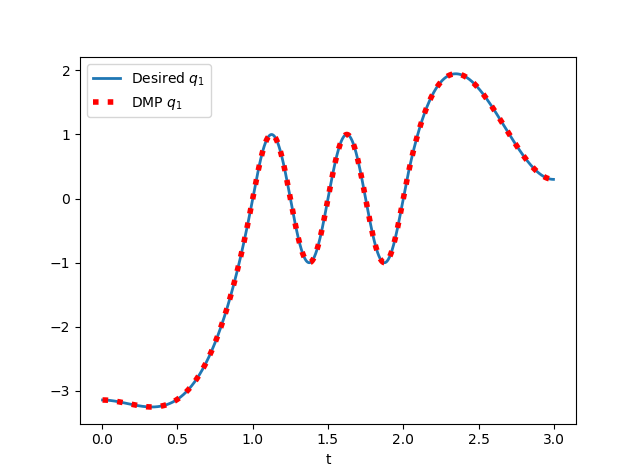
\includegraphics[width=\linewidth]{img/2c-q1.png}
		\captionof{figure}[trajecotry q2]{The desired and reproduced trajectory of $q_1$ are nearly equal.}
		\label{fig:q1_des}
	\end{minipage}
	\hfill
	\begin{minipage}{0.45\linewidth} 
		\centering
		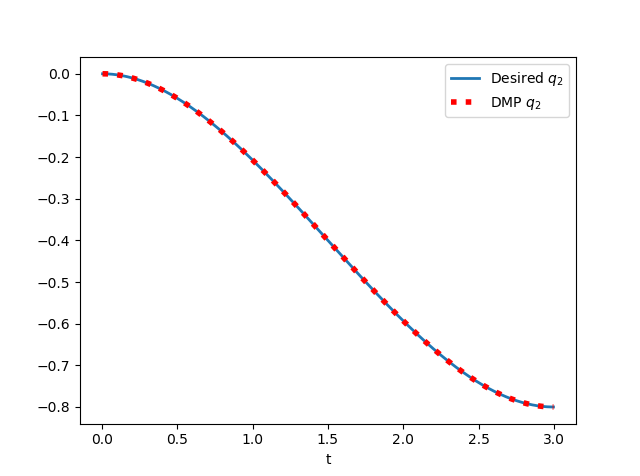
\includegraphics[width=\linewidth]{img/2c-q2.png}
		\captionof{figure}[Trajectory q2]{The desired and reproduced trajectory of $q_2$ are also nearly equal.}
		\label{fig:q2_des}
	\end{minipage}
\end{center}

You can use this functions to reproduce the demonstration trajectory. In figure \ref{fig:q1_des} and figure \ref{fig:q2_des} you can see, that the desired trajectory and the reproduced trajectory from the DMP are nearly the same. This is a good result and shows that we use enough basis functions.

\end{answer}

\end{question}

%----------------------------------------------

\begin{question}{Double Pendulum - Conditioning on the Final Position}{3}
Using the trained DMPs from the previous question, simulate the system with different goal positions: first with $q_{t=\mathrm{end}} = \{0, 0.2\}$ and then with $q_{t=\mathrm{end}} = \{0.8, 0.5\}$. Generate one figure per DoF. In each figure, plot the demonstrated trajectory and the reproduced trajectories with different goal positions.
How do you interpret the result? 

\begin{answer}
In this task we use the trained DMP from question c) with a different goal position. You get the trajectories in figure \ref{fig:q1_new_goal} and figure \ref{fig:q2_new_goal}. The trajectories of q1 are most of the time nearly the same, the new trajectory is only shifted a bit up or down. The only really difference is the start behavior. All trajectories start at the same point, but then the reach the offset to the trained DMP really fast. This is not an optimal behavior, because it would be more useful, if the new trajectory follows the trained one at the beginning and than slowly moves away from it.

The $q_2$-trajectory looks really different compared to the trained DMP. It rises very fast at the beginning and after this it shows the same course like the trained DMP, but has a big offset. It is hard to interpret the graph without some more graphical simulation, but this high gradient at the beginning cannot be good for the robot.

\begin{center}
	\begin{minipage}{0.45\linewidth} 
		\centering
		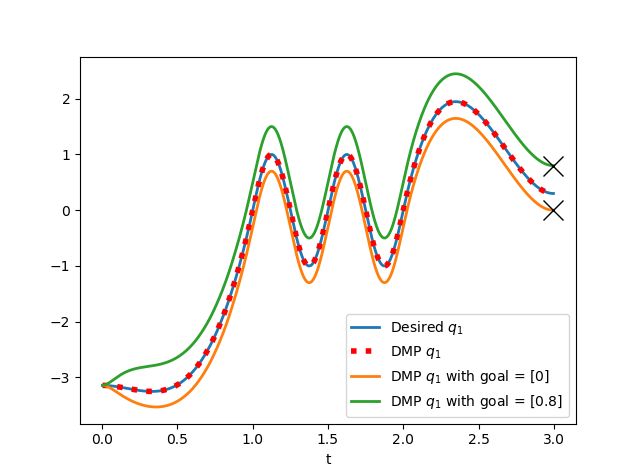
\includegraphics[width=\linewidth]{img/2d-q1.png}
		\captionof{figure}[trajecotry q2]{$q_1$ with goal position $q_{t=\mathrm{end}} = \{0, 0.2\}$.}
		\label{fig:q1_new_goal}
	\end{minipage}
	\hfill
	\begin{minipage}{0.45\linewidth} 
		\centering
		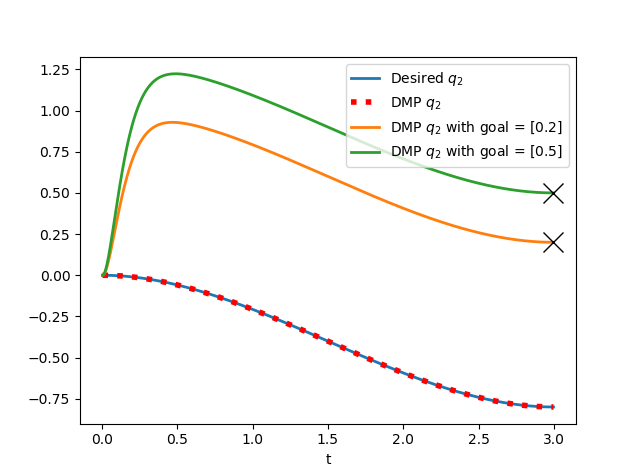
\includegraphics[width=\linewidth]{img/2d-q2.png}
		\captionof{figure}[Trajectory q2]{$q_2$ with goal position $q_{t=\mathrm{end}} = \{0.8, 0.5\}$.}
		\label{fig:q2_new_goal}
	\end{minipage}
\end{center}
\end{answer}


\end{question}

%----------------------------------------------

\begin{question}{Double Pendulum - Temporal Modulation}{3}
Using the trained DMPs from the previous question, simulate the system with different temporal scaling factors $\tau=\{0.5, 1.5\}$. Generate one figure per DoF and explain the result.

\begin{answer}
	
Now the DMP is rescaled in the time. One trajectory is faster as the trained DMP, one is slower. You can see the result in figure~\ref{fig:q1_new_t} and figure~\ref{fig:q2_new_t}. The trajectories follow the same course, but have different time scalings. It looks like a linear rescaling of the trained DMP.
Note that in this example the trained and temporal scaled trajectories have the same goal as the desired trajectory. If the temporal scaling factor is smaller than 1 the goal position is not reached. If the temporal scaling factor is higher than one the goal position is reached faster.

\begin{center}
	\begin{minipage}{0.45\linewidth} 
		\centering
		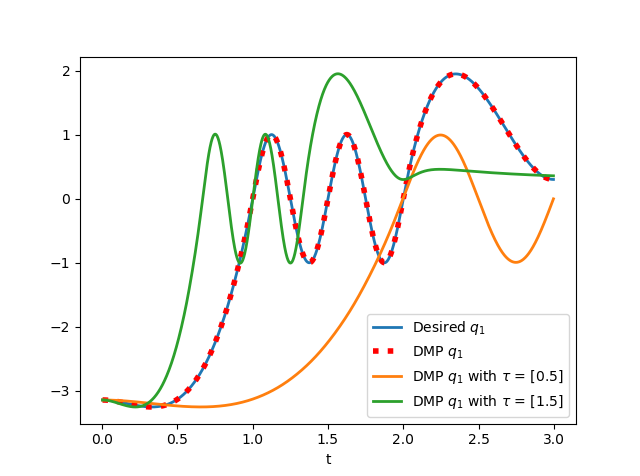
\includegraphics[width=\linewidth]{img/2f-q1.png}
		\captionof{figure}[trajecotry q2]{$q_1$ with different end times.}
		\label{fig:q1_new_t}
	\end{minipage}
	\hfill
	\begin{minipage}{0.45\linewidth} 
		\centering
		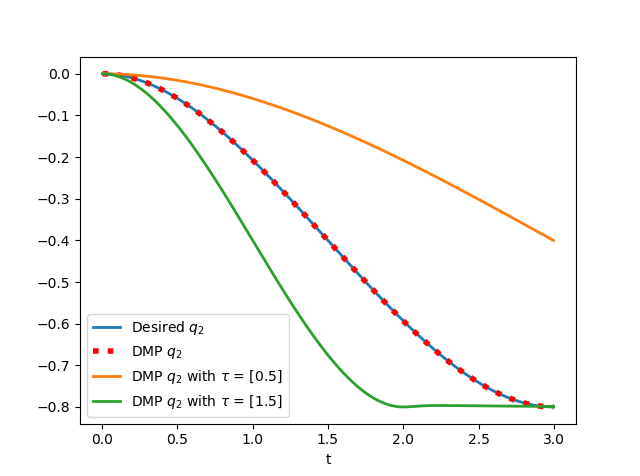
\includegraphics[width=\linewidth]{img/2f-q2.png}
		\captionof{figure}[Trajectory q2]{$q_2$ with different end times}
		\label{fig:q2_new_t}
	\end{minipage}
\end{center}
\end{answer}


\end{question}

%----------------------------------------------

\begin{question}[bonus]{Probabilistic Movement Primitives - Radial Basis Function}{3}
We now want to use ProMPs. Before we train them, we need to define some basis functions. We decide to use $N = 30$ radial basis functions (RBFs) with centers uniformly distributed in the time interval $[0-2b,T+2b]$, where $T$ is the end time of the demonstrations.
The bandwidth of the Gaussian basis (std) is set to $b=0.2$. 
Implement these basis functions in \texttt{getProMPBasis.py}. 
Do not forget to normalize the basis such at every time-point they sum-up to one! Attach a plot showing the basis functions in time and a snippet of your code. 

\begin{answer}

\begin{center}
	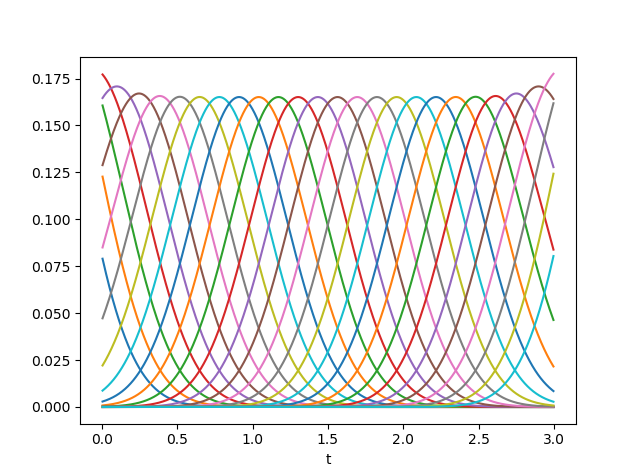
\includegraphics[width=0.6\linewidth]{img/2f.png}
	\captionof{figure}{30 uniformly distributed gaussian basis functions.}
	\label{fig:gaussian_basis}
\end{center}

\lstinputlisting{code/getProMPBasis.py}
\end{answer}
\end{question}

%----------------------------------------------

\begin{question}[bonus]{Probabilistic Movement Primitives - Training}{7}
In this exercise you will train the ProMPs using the imitation learning data from \texttt{getImitationData.py} and the RBFs defined in the previous question. Modify the \texttt{proMP.py} in order to estimate weight vectors $w_i$ reproducing the different demonstrations. Then, fit a Gaussian using all the weight vectors. Generate a plot showing the desired trajectory distribution in time (mean and std) as well as the trajectories used for imitation. Attach a snippet of your code.  

\begin{answer}
\begin{center}
	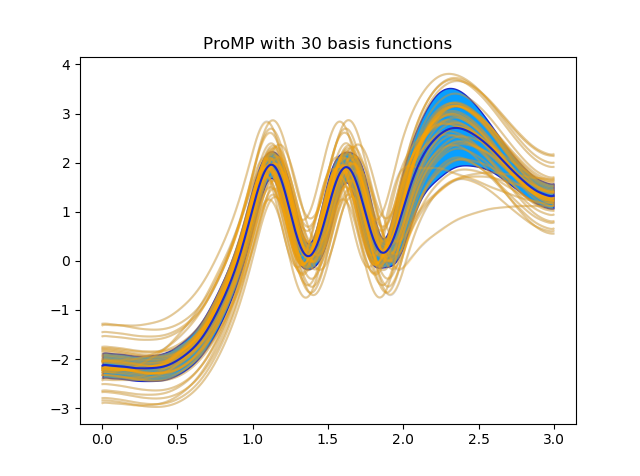
\includegraphics[width=.7\linewidth]{img/2g.png}
	\captionof{figure}{In this figure you can see the trained ProMP in blue. The dark blue line shows the mean, the light blue area is the uncertainty. The grey lines are the training data and the orange lines are the reproduced trajectories.  }
\end{center}

\lstinputlisting{code/proMP_h.py}

\end{answer}

\end{question}

%----------------------------------------------

\begin{question}[bonus]{Probabilistic Movement Primitives - Number of Basis Functions}{2}
Evaluate the effects of using a reduced number of RBFs. Generate two plots showing the desired trajectory distribution and the trajectories used for imitation as in the previous exercise, but this time use $N=20$ and $N=10$ basis functions. Briefly analyze your results.

\begin{answer}
\begin{center}
	\begin{minipage}{0.49\linewidth}
		\centering
		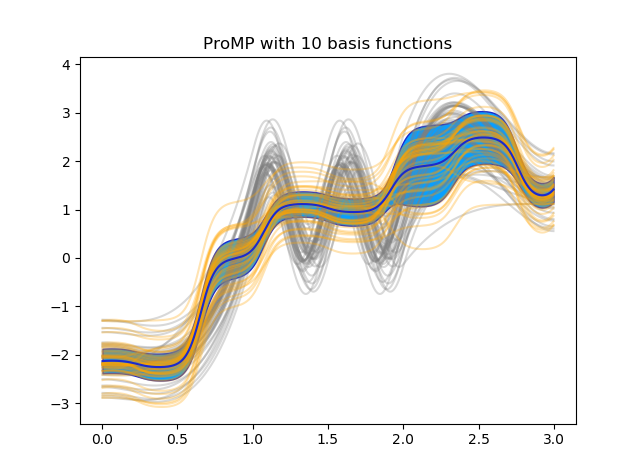
\includegraphics[width=1\linewidth]{img/2h_10.png}
		\captionof{figure}{ProMP with 10 basis functions: The reproduced trajectories cannot follow the training trajectories, they only show the mean. This is not a usefull model.}
		\label{fig:proMP10}
	\end{minipage}
	\hfill
	\begin{minipage}{0.49\linewidth}
		\centering
		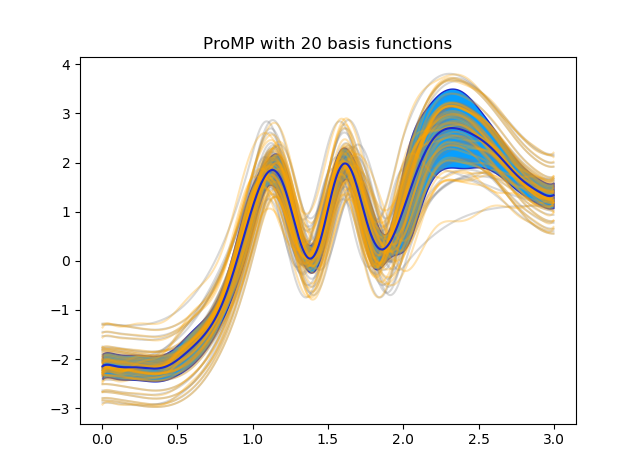
\includegraphics[width=1\linewidth]{img/2h_20.png}
		\captionof{figure}{ProMp with 20 basis functions: This ProMP is very simluar to the ProMP with 30 basis function. So this is also a good model. Then you look at the single training trajectories, you can see some dfferences between the training and the reproduced trajectory. Because of this some more basis functions would be usefull.}
		\label{fig:proMP20}
	\end{minipage}
\end{center}
\end{answer}

\end{question}

%----------------------------------------------


\begin{question}[bonus]{Probabilistic Movement Primitives - Conditioning}{4}
Using Gaussian conditioning calculate the new distribution over the weight vectors $w_i$ such as the trajectory has a via point at position $y^*=3$ at time $t_\textrm{cond}=1150$ with variance $\Sigma_{y^*}=0.0002$. Use again 30 basis functions.
Assuming that the probability over the weights is given by $\mathcal{N}(\vec w|\vec \mu_w,\vec \Sigma_w)$ and the probability of being to that position is given by $\mathcal{N}(y^*|\vec \Phi \vec w, \Sigma_{y^*} )$, show how the new distribution over $\vec w$ is computed (how does the mean and variance look like)?
\\
Then, in a single plot, show the previous distribution (learned from imitation) and the new distribution (after conditioning). Additionally, sample $K=10$ random weight vectors from the ProMP, compute the trajectories and plot them in the same plot. Analyze briefly your results and attach a snippet of your code.

\begin{answer}
\begin{center}
	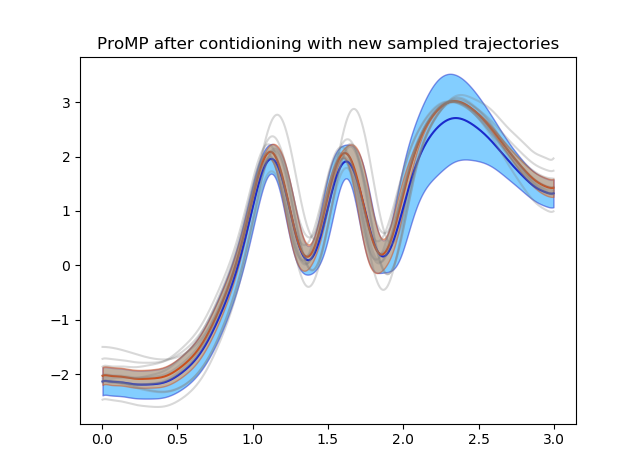
\includegraphics[width=0.7\linewidth]{img/2i.png}
	\captionof{figure}{New distribution after reconditioning: The bule line shows the original ProMp, the orange one is the conditioned ProMp. The grey functions are example trajectories.}
	\label{fig:newProMP}
\end{center}

Figure~\ref{fig:newProMP} shows the conditioned ProMP. You can see original ProMp in blue and the new one in orange. The mean of the new ProMp goes exactly through the given point at $t_\textrm{cond}=1150$. The uncertainty at this point is very low. Then you look at other points of the ProMp the uncertainty is much bigger. The new trajectory follows the original ProMp most of the time and only at the given position it moves away from it. This is a much better behavior as the DMP in the last exercise.

\lstinputlisting{code/proMP_i.py}
\end{answer}

\end{question}

\end{questions}
